\documentclass[paper=a4, fontsize=11pt]{scrartcl}\usepackage[]{graphicx}\usepackage[]{color}
%% maxwidth is the original width if it is less than linewidth
%% otherwise use linewidth (to make sure the graphics do not exceed the margin)
\makeatletter
\def\maxwidth{ %
  \ifdim\Gin@nat@width>\linewidth
    \linewidth
  \else
    \Gin@nat@width
  \fi
}
\makeatother

\definecolor{fgcolor}{rgb}{0.345, 0.345, 0.345}
\newcommand{\hlnum}[1]{\textcolor[rgb]{0.686,0.059,0.569}{#1}}%
\newcommand{\hlstr}[1]{\textcolor[rgb]{0.192,0.494,0.8}{#1}}%
\newcommand{\hlcom}[1]{\textcolor[rgb]{0.678,0.584,0.686}{\textit{#1}}}%
\newcommand{\hlopt}[1]{\textcolor[rgb]{0,0,0}{#1}}%
\newcommand{\hlstd}[1]{\textcolor[rgb]{0.345,0.345,0.345}{#1}}%
\newcommand{\hlkwa}[1]{\textcolor[rgb]{0.161,0.373,0.58}{\textbf{#1}}}%
\newcommand{\hlkwb}[1]{\textcolor[rgb]{0.69,0.353,0.396}{#1}}%
\newcommand{\hlkwc}[1]{\textcolor[rgb]{0.333,0.667,0.333}{#1}}%
\newcommand{\hlkwd}[1]{\textcolor[rgb]{0.737,0.353,0.396}{\textbf{#1}}}%

\usepackage{framed}
\makeatletter
\newenvironment{kframe}{%
 \def\at@end@of@kframe{}%
 \ifinner\ifhmode%
  \def\at@end@of@kframe{\end{minipage}}%
  \begin{minipage}{\columnwidth}%
 \fi\fi%
 \def\FrameCommand##1{\hskip\@totalleftmargin \hskip-\fboxsep
 \colorbox{shadecolor}{##1}\hskip-\fboxsep
     % There is no \\@totalrightmargin, so:
     \hskip-\linewidth \hskip-\@totalleftmargin \hskip\columnwidth}%
 \MakeFramed {\advance\hsize-\width
   \@totalleftmargin\z@ \linewidth\hsize
   \@setminipage}}%
 {\par\unskip\endMakeFramed%
 \at@end@of@kframe}
\makeatother

\definecolor{shadecolor}{rgb}{.97, .97, .97}
\definecolor{messagecolor}{rgb}{0, 0, 0}
\definecolor{warningcolor}{rgb}{1, 0, 1}
\definecolor{errorcolor}{rgb}{1, 0, 0}
\newenvironment{knitrout}{}{} % an empty environment to be redefined in TeX

\usepackage{alltt}
\newtheorem{thm}{\textbf{Theorem}}[section]
\newtheorem{prop}{\textbf{Proposition}}[section]
\newtheorem{defn}{\textbf{Definition}}[section]
\newtheorem{claim}{\textbf{Claim}}[section]
\newtheorem{lemma}{\textbf{Lemma}}[section]
\usepackage{amssymb,latexsym,amsmath}
\usepackage{epsfig}
\usepackage{caption}
\usepackage{color}
\usepackage{float}
\usepackage{fullpage}
\linespread{1.3}
\usepackage[titletoc]{appendix}
\usepackage{chngcntr}
\usepackage{multirow}
\usepackage{parskip}					%for no indent
\usepackage[authoryear]{natbib}			%for nice references
\usepackage{listings}		% for R code
\usepackage{epstopdf}
%\usepackage[nottoc,numbib]{tocbibind}
\captionsetup{font=scriptsize,labelfont=scriptsize}	%makes all captions tiny size
\IfFileExists{upquote.sty}{\usepackage{upquote}}{}

\begin{document}

This code visualizes trades and the top of the order book for US 10Y Treasuries on 2012-10-26 using
clock time and tick time. The mid price and micro prices are also graphed versus tick time.
Figure \ref{fig:ticktime} below shows the graph generated for the order book with respect to tick
time.

\begin{figure}[H]
\begin{center}
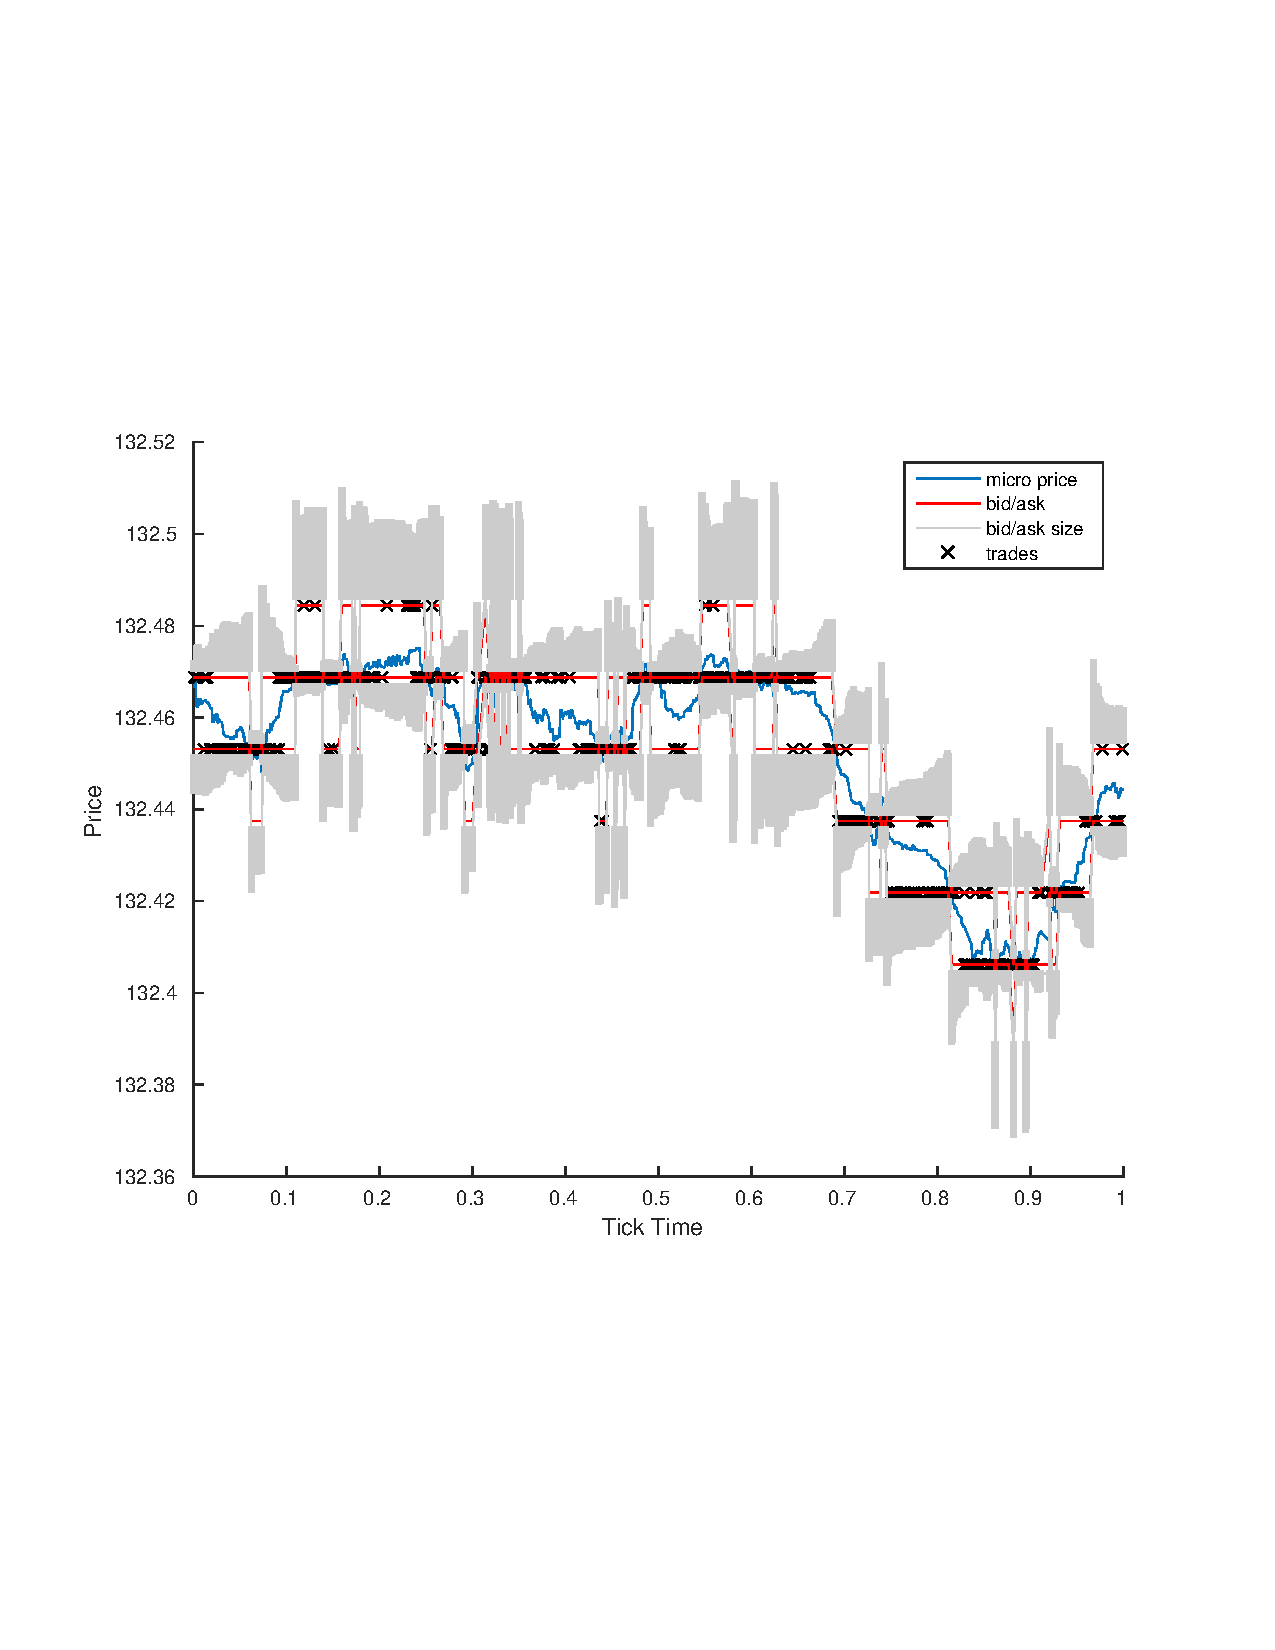
\includegraphics[height=9cm, width=12cm, trim=4cm 7cm 4cm 7cm]{ticktime.pdf}
\caption{US 10YR Future Order Book}
\label{fig:ticktime}
\end{center}
\end{figure}

Exogenous market impact effects are investigated by regressing changes in the micro price on to
lagged signed trades, shown in Equation \ref{eq:1}. The assumption is made that if the transacted trade price is closer to the bid then the trade is a sale and similarly if the transacted trade price is closer to the ask then the trade is a buy.

\begin{align} \label{eq:1}
\Delta P_{\kappa} = \beta_{1}\Delta Sgn Q_{\kappa - 1} + ... + \beta_{10}\Delta Sgn Q_{\kappa - 10} + \epsilon_{\kappa}
\end{align}

The $R^2$ of this model is 0.0737 which is a large improvement over a model including only 1 lag, which has an $R^2$ of 0.0178. Both sets of residuals exhibit significant autocorrelation indicating further improvement could likely be made through fitting some form of ARIMA model.

\end{document}
